\documentclass{beamer}
\usetheme{Dresden}
\usecolortheme{whale}
\usepackage[utf8]{inputenc}
\usepackage[T1]{fontenc}
\usepackage{ragged2e}
\usepackage{amssymb}
\usepackage{booktabs}
\usepackage{graphicx}
\usepackage{mathtools}
\usepackage{commath}
\usepackage{amsmath}
\usepackage{wrapfig}
\usepackage{multicol}
\usepackage{listings}
\usepackage{tikz}
\usetikzlibrary{arrows.meta, positioning, shapes.geometric, shapes.symbols, fit, backgrounds, calc}

\newcommand{\nt}{$\underline{\text{Note}}:$ }
\newcommand{\ex}{$\underline{\text{Example}}:$ }
\newcommand{\rem}{$\underline{\text{Recall}}:$ }
\newcommand{\rmk}{$\underline{\text{Remark}}:$ }
\newcommand{\tab}{\quad}
\newcommand{\nll}{\\\vspace{2ex}}

\graphicspath{ {images/} }

\lstset{
    basicstyle=\ttfamily\scriptsize,
    keywordstyle=\color{blue!70!black},
    commentstyle=\color{gray},
    breaklines=true,
    frame=single,
    backgroundcolor=\color{gray!5},
}

\title[Voice Scribe v2]{Voice Scribe v2\\Local-First Speech-to-Text for Development Workflows}
\author[J. Yanez]{Johnraymond Yanez}
\institute[Voice Scribe]{Voice Scribe}
\date{\today}

\begin{document}


% -- Title -----------------------------------------------------------------
\begin{frame}
\small{\titlepage}
\end{frame}


% -- Outline ---------------------------------------------------------------
\begin{frame}{Overview}
    \begin{itemize}
        \item \textbf{Motivation} --- Why local transcription for developer workflows?
        \item \textbf{Architecture} --- Two-service system over localhost
        \item \textbf{Container Strategy} --- GPU passthrough, model caching, isolation
        \item \textbf{Audio Pipeline} --- Browser recording through inference
        \item \textbf{Frontend} --- React component tree and state machine
        \item \textbf{Security} --- Threat model, privacy, operational telemetry
        \item \textbf{Development} --- Workflow, tooling, and testing
        \item \textbf{Roadmap} --- v1 scope and what comes next
    \end{itemize}
\end{frame}


% =========================================================================
\section{Motivation}
% =========================================================================

\begin{frame}{The Problem}
    \small
    Developer workflows increasingly involve AI coding assistants ---
    tools where natural language is the primary input.

    \vspace{0.2em}
    \begin{columns}[T]
        \begin{column}{0.48\textwidth}
            \textbf{Friction points}
            \begin{itemize}\setlength{\itemsep}{0pt}\setlength{\parskip}{0pt}
                \item Typing long prompts breaks flow
                \item Context-switching between thinking and typing
                \item Cloud transcription raises privacy concerns
                \item Existing tools not optimized for dev use cases
            \end{itemize}
        \end{column}
        \begin{column}{0.48\textwidth}
            \textbf{What we want}
            \begin{itemize}\setlength{\itemsep}{0pt}\setlength{\parskip}{0pt}
                \item Speak naturally, get text
                \item Text stays on your machine
                \item One-click copy into any tool
                \item No accounts, no cloud, no latency
            \end{itemize}
        \end{column}
    \end{columns}

    \vspace{0.2em}
    \begin{block}{Core Insight}
        Speech is the fastest way to externalize a thought.
        The bottleneck is getting that speech into text \textit{locally}
        with sufficient accuracy.
    \end{block}
\end{frame}


\begin{frame}{Design Principles}
    Four principles govern every v1 decision:

    \vspace{0.6em}
    \begin{enumerate}
        \item \textbf{Local-first}\\
              Audio and transcripts stay on the user's machine.
              No cloud services required at any point.

        \vspace{0.3em}
        \item \textbf{Host for interaction, container for inference}\\
              The browser owns mic access, clipboard, and editing.
              The container owns model loading and GPU inference.

        \vspace{0.3em}
        \item \textbf{Audio is transient, text is durable}\\
              Raw audio is short-lived input --- deleted after processing.
              The transcript is the user-facing artifact.

        \vspace{0.3em}
        \item \textbf{Scope matches the milestone}\\
              Repo structure and services reflect v1 reality,
              not v3 aspirations. Architecture stays flat until
              complexity is earned.
    \end{enumerate}
\end{frame}


% =========================================================================
\section{Architecture}
% =========================================================================

\begin{frame}{System Architecture}
    \small
    Voice Scribe is a two-service system communicating over localhost HTTP.

    \vspace{0.3em}
    \begin{itemize}\setlength{\itemsep}{2pt}
        \item The \textbf{frontend} runs on the host --- it owns browser APIs
              (microphone, clipboard, DOM) that cannot exist inside a container
        \item The \textbf{backend} runs in a Docker container --- it owns
              GPU-accelerated inference via CUDA, which cannot run in a browser
        \item Communication is plain HTTP. No WebSocket, no reverse proxy,
              no message queue
        \item Both services bind to \texttt{localhost} only --- never
              network-accessible
    \end{itemize}

    \vspace{0.2em}
    \begin{block}{}
        The split is dictated by hardware constraints, not architectural
        preference. Each service does what only it can do.
    \end{block}
\end{frame}


\begin{frame}{System Architecture --- Diagram}
    \begin{center}
    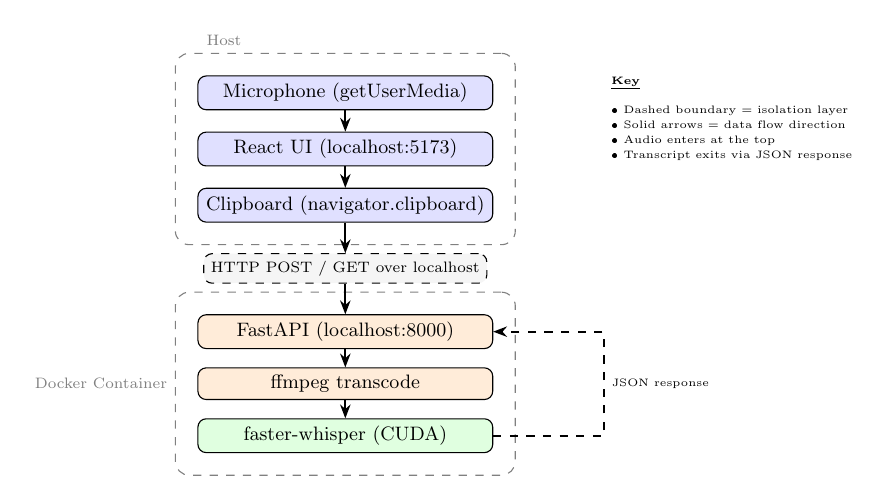
\begin{tikzpicture}[scale=0.78, every node/.style={transform shape},
        node distance=0.3cm,
        box/.style={draw, rounded corners=3pt, minimum width=4.8cm,
                    minimum height=0.45cm, font=\small, align=center},
        host/.style={box, fill=blue!12},
        container/.style={box, fill=orange!15},
        runtime/.style={box, fill=green!12},
        httpbox/.style={draw, rounded corners=3pt, minimum width=3.8cm,
                    minimum height=0.45cm, font=\scriptsize, align=center,
                    fill=gray!8, dashed},
        arr/.style={-{Stealth[length=5pt]}, thick},
        lbl/.style={font=\scriptsize, text=gray},
        boundary/.style={draw, dashed, rounded corners=5pt, gray,
                         inner sep=8pt},
    ]
        % Host boundary
        \node[host] (mic) {Microphone (getUserMedia)};
        \node[host, below=0.35cm of mic] (ui) {React UI (localhost:5173)};
        \node[host, below=0.35cm of ui] (clip) {Clipboard (navigator.clipboard)};

        \begin{scope}[on background layer]
            \node[boundary, fit=(mic)(ui)(clip),
                  label={[font=\scriptsize, text=gray]above left:Host}] {};
        \end{scope}

        % Connection — distinct visual layer between boundaries
        \node[httpbox] (http) [below=0.5cm of clip]
              {HTTP POST / GET over localhost};

        % Container boundary
        \node[container, below=0.5cm of http] (api) {FastAPI (localhost:8000)};
        \node[container, below=0.3cm of api] (ffmpeg) {ffmpeg transcode};
        \node[runtime, below=0.3cm of ffmpeg] (whisper) {faster-whisper (CUDA)};

        \begin{scope}[on background layer]
            \node[boundary, fit=(api)(ffmpeg)(whisper),
                  label={[font=\scriptsize, text=gray]left:Docker Container}] {};
        \end{scope}

        % Arrows — host internal flow
        \draw[arr] (mic) -- (ui);
        \draw[arr] (ui) -- (clip);

        % Arrow from clip down to HTTP, then HTTP down to API
        \draw[arr] (clip) -- (http);
        \draw[arr] (http) -- (api);

        % Container internal flow
        \draw[arr] (api) -- (ffmpeg);
        \draw[arr] (ffmpeg) -- (whisper);

        % JSON response path — loop back with clearance
        \draw[arr, dashed] (whisper.east) -- ++(1.8,0)
              |- node[near start, right, font=\tiny]{JSON response} (api.east);

        % Key — top-right corner where there is open space
        \node[anchor=north west, font=\tiny\bfseries]
              (keytitle) at ([xshift=1.8cm, yshift=0.1cm]mic.north east)
              {\underline{Key}};
        \node[anchor=north west, text width=4.0cm, font=\tiny,
              align=left, below=0.02cm of keytitle.south west, anchor=north west] {%
            \textbullet\ Dashed boundary = isolation layer\\[1pt]
            \textbullet\ Solid arrows = data flow direction\\[1pt]
            \textbullet\ Audio enters at the top\\[1pt]
            \textbullet\ Transcript exits via JSON response};
    \end{tikzpicture}
    \end{center}
\end{frame}


\begin{frame}{Tech Stack}
    \begin{table}
    \centering\small
    \begin{tabular}{@{} p{1.5cm} p{3.6cm} p{4.8cm} @{}}
        \toprule
        \textbf{Layer} & \textbf{Technology} & \textbf{Rationale} \\
        \midrule
        Frontend   & React, TypeScript, Vite  & Mic access, clipboard, fast iteration \\
        Backend    & Python, FastAPI           & Model ecosystem, easy containerization \\
        STT Engine & faster-whisper (large-v3) & Accuracy/speed on local GPU \\
        Transcode  & ffmpeg (in container)     & Normalizes browser audio to WAV \\
        Container  & Docker, CUDA 12.6         & GPU isolation, reproducibility \\
        \bottomrule
    \end{tabular}
    \end{table}

    \vspace{0.4em}
    \begin{block}{Selection Principle}
        Each layer is selected for its ecosystem strength at that boundary.
        React for browser APIs, Python for ML inference, Docker for GPU
        isolation. No layer is forced to do work outside its strength.
    \end{block}
\end{frame}


\begin{frame}{Request Lifecycle}
    A single transcription request passes through eight stages.
    The frontend handles stages 1 and 8; the backend handles 2--7.

    \vspace{0.6em}
    \begin{itemize}
        \item \textbf{Validation} (stages 2--3) rejects bad input early ---
              before any expensive I/O or computation
        \item \textbf{Processing} (stages 4--6) is the core pipeline:
              temp file, transcode, inference
        \item \textbf{Cleanup} (stage 7) is guaranteed by \texttt{try/finally}
              --- both temp files are deleted on success \textit{and} failure
        \item Every stage between 3--7 is bounded by explicit limits:
              10\,MB upload, 60\,s duration, 30\,s ffmpeg timeout
    \end{itemize}

    \vspace{0.4em}
    \nt The synchronous design means the HTTP connection stays open
    during inference. For v1's single-user use case, this is correct.
\end{frame}


\begin{frame}{Request Lifecycle --- Diagram}
    \begin{center}
    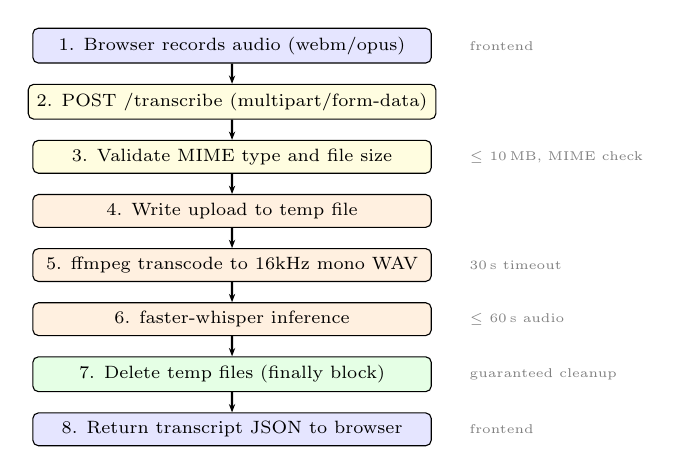
\begin{tikzpicture}[scale=0.92, every node/.style={transform shape},
        node distance=0.28cm,
        stepbox/.style={draw, rounded corners=2pt, minimum width=5.5cm,
                     minimum height=0.38cm, font=\scriptsize, align=center},
        fe/.style={stepbox, fill=blue!10},
        val/.style={stepbox, fill=yellow!12},
        proc/.style={stepbox, fill=orange!12},
        clean/.style={stepbox, fill=green!10},
        arr/.style={-{Stealth[length=3pt]}, thick},
        brace/.style={decorate, decoration={brace, amplitude=4pt, mirror}},
        lbl/.style={font=\tiny, text=gray},
    ]
        \node[fe]    (s1) {1. Browser records audio (webm/opus)};
        \node[val,   below=of s1] (s2) {2. POST /transcribe (multipart/form-data)};
        \node[val,   below=of s2] (s3) {3. Validate MIME type and file size};
        \node[proc,  below=of s3] (s4) {4. Write upload to temp file};
        \node[proc,  below=of s4] (s5) {5. ffmpeg transcode to 16kHz mono WAV};
        \node[proc,  below=of s5] (s6) {6. faster-whisper inference};
        \node[clean, below=of s6] (s7) {7. Delete temp files (finally block)};
        \node[fe,    below=of s7] (s8) {8. Return transcript JSON to browser};

        \foreach \a/\b in {s1/s2, s2/s3, s3/s4, s4/s5, s5/s6, s6/s7, s7/s8} {
            \draw[arr] (\a) -- (\b);
        }

        % Side labels
        \node[lbl, right=0.4cm of s1] {frontend};
        \node[lbl, right=0.4cm of s3] {$\le$ 10\,MB, MIME check};
        \node[lbl, right=0.4cm of s5] {30\,s timeout};
        \node[lbl, right=0.4cm of s6] {$\le$ 60\,s audio};
        \node[lbl, right=0.4cm of s7] {guaranteed cleanup};
        \node[lbl, right=0.4cm of s8] {frontend};
    \end{tikzpicture}
    \end{center}

    \vspace{0.1em}
    {\scriptsize \textcolor{blue!60}{Blue} = frontend,
    \textcolor{yellow!70!black}{Yellow} = validation,
    \textcolor{orange!70}{Orange} = processing,
    \textcolor{green!50!black}{Green} = cleanup.}
\end{frame}


% =========================================================================
\section{Container Strategy}
% =========================================================================

\begin{frame}{Host vs.\ Container Responsibilities}
    \small
    The boundary between host and container is drawn by hardware capability.

    \vspace{0.3em}
    \begin{columns}[T]
        \begin{column}{0.48\textwidth}
            \textbf{Host (Browser)}
            \begin{itemize}\setlength{\itemsep}{0pt}
                \item Microphone access
                \item Audio recording
                \item User interface rendering
                \item Text editing
                \item Clipboard access
                \item Codec negotiation
            \end{itemize}
        \end{column}
        \begin{column}{0.48\textwidth}
            \textbf{Container (Docker)}
            \begin{itemize}\setlength{\itemsep}{0pt}
                \item Model weight management
                \item Audio transcoding (ffmpeg)
                \item GPU inference (faster-whisper)
                \item MIME validation
                \item Temp file lifecycle
                \item Structured logging
            \end{itemize}
        \end{column}
    \end{columns}

    \vspace{0.3em}
    Browser APIs (mic, clipboard) cannot run in a container.
    GPU inference cannot run efficiently in a browser.
    The container is disposable --- only the model cache
    and the transcript text survive beyond a single session.
\end{frame}


\begin{frame}{GPU Passthrough}
    \small
    Voice Scribe uses NVIDIA GPU passthrough from Windows through
    four layers. Each layer must be correctly configured for the
    next to function.

    \vspace{0.3em}
    \begin{itemize}\setlength{\itemsep}{2pt}
        \item \textbf{Windows NVIDIA driver} provides CUDA to the WSL2 kernel
        \item \textbf{WSL2 kernel} bridges GPU access into Linux userspace
        \item \textbf{Docker Desktop} (WSL2 backend) exposes the GPU to containers
        \item \textbf{Docker Compose} \texttt{deploy.resources} reserves the device
    \end{itemize}

    \vspace{0.2em}
    This is the highest-risk setup step in the entire project.
    A misaligned driver version, WSL kernel, or Docker Desktop setting
    breaks the chain silently.

    \vspace{0.2em}
    \nt The bootstrap script \texttt{ops/scripts/bootstrap\_gpu\_check.sh}
    gates all development behind GPU verification. Do not write
    application code until it passes.
\end{frame}


\begin{frame}{GPU Passthrough --- Diagram}
    \begin{center}
    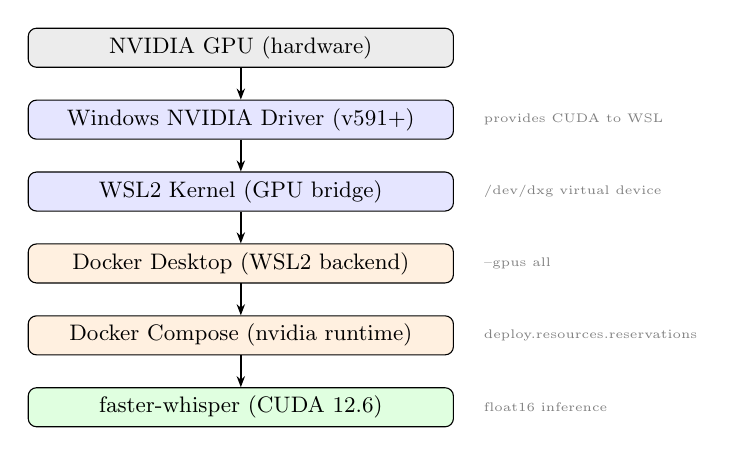
\begin{tikzpicture}[scale=0.9, every node/.style={transform shape},
        node distance=0.45cm,
        layer/.style={draw, rounded corners=3pt, minimum width=6cm,
                      minimum height=0.5cm, font=\small, align=center},
        hw/.style={layer, fill=gray!15},
        os/.style={layer, fill=blue!10},
        dock/.style={layer, fill=orange!12},
        app/.style={layer, fill=green!12},
        arr/.style={-{Stealth[length=4pt]}, thick},
        lbl/.style={font=\tiny, text=gray},
    ]
        \node[hw]   (gpu)    {NVIDIA GPU (hardware)};
        % TODO: replace v591+ with the specific driver version validated by the team
        %       and append the validation date, e.g. {Windows NVIDIA Driver (v591.43, validated 2026-MM-DD)}
        %       Principal's note: "591+ will mean something different six months from now."
        \node[os,   below=of gpu]   (driver) {Windows NVIDIA Driver (v591+)};
        \node[os,   below=of driver](wsl)    {WSL2 Kernel (GPU bridge)};
        \node[dock, below=of wsl]   (docker) {Docker Desktop (WSL2 backend)};
        \node[dock, below=of docker](compose){Docker Compose (nvidia runtime)};
        \node[app,  below=of compose](app)   {faster-whisper (CUDA 12.6)};

        \draw[arr] (gpu) -- (driver);
        \draw[arr] (driver) -- (wsl);
        \draw[arr] (wsl) -- (docker);
        \draw[arr] (docker) -- (compose);
        \draw[arr] (compose) -- (app);

        % Annotations
        \node[lbl, right=0.3cm of driver] {provides CUDA to WSL};
        \node[lbl, right=0.3cm of wsl]    {/dev/dxg virtual device};
        \node[lbl, right=0.3cm of docker]  {--gpus all};
        \node[lbl, right=0.3cm of compose] {deploy.resources.reservations};
        \node[lbl, right=0.3cm of app]     {float16 inference};
    \end{tikzpicture}
    \end{center}

    \vspace{0.2em}
    {\scriptsize Each layer depends on the one above it. The bootstrap check
    verifies the full chain by running \texttt{nvidia-smi} inside a
    GPU-enabled container.}
\end{frame}


\begin{frame}{Model Caching}
    The \texttt{large-v3} model is $\sim$3\,GB. It downloads once
    from HuggingFace and must persist across container restarts.

    \vspace{0.6em}
    \begin{itemize}
        \item Model weights are \textbf{not} baked into the Docker image ---
              this would bloat the image and prevent model swaps
        \item A host-mounted volume (\texttt{data/cache/}) maps to
              \texttt{/cache} inside the container
        \item First run: $\sim$60\,s download. Subsequent runs: $< 2$\,s load
        \item \texttt{data/cache/} is gitignored --- weights never enter the repo
    \end{itemize}

    \vspace{0.4em}
    \rmk The compose file sets \texttt{user: \$\{UID\}:\$\{GID\}} so
    cache files are owned by the host user, avoiding permission
    mismatches between container and host filesystems.
\end{frame}


\begin{frame}{Model Caching --- Diagram}
    \begin{center}
    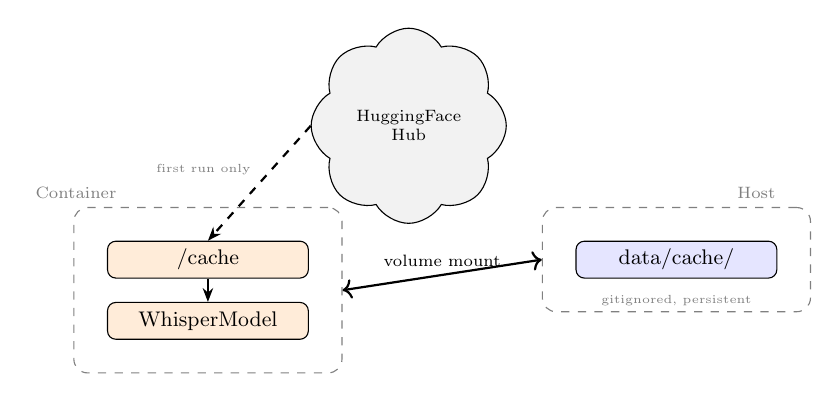
\begin{tikzpicture}[scale=0.85, every node/.style={transform shape},
        node distance=0.4cm,
        box/.style={draw, rounded corners=3pt, minimum width=3cm,
                    minimum height=0.55cm, font=\small, align=center},
        cbox/.style={box, fill=orange!15},
        hbox/.style={box, fill=blue!10},
        cloudnode/.style={draw, cloud, cloud puffs=8, cloud puff arc=120,
                      minimum width=2.2cm, minimum height=1cm,
                      font=\scriptsize, align=center, fill=gray!10},
        arr/.style={-{Stealth[length=5pt]}, thick},
        lbl/.style={font=\tiny, text=gray},
        boundary/.style={draw, dashed, rounded corners=5pt, gray, inner sep=12pt},
    ]
        % HuggingFace — top center, clearly above both boundaries
        \node[cloudnode] (hf) at (3.0, 2.0) {HuggingFace\\Hub};

        % Container — /cache on top so HuggingFace arrow drops cleanly to it
        \node[cbox] (cache) at (0, 0) {/cache};
        \node[cbox, below=0.35cm of cache] (model) {WhisperModel};

        \begin{scope}[on background layer]
            \node[boundary, fit=(cache)(model),
                  label={[font=\scriptsize, text=gray]above left:Container}] (cbound) {};
        \end{scope}

        % Host — pushed right so volume mount label has clear air
        \node[hbox] (hostcache) at (7.0, 0) {data/cache/};
        \node[lbl, below=0.12cm of hostcache] {gitignored, persistent};

        \begin{scope}[on background layer]
            \node[boundary, fit=(hostcache),
                  label={[font=\scriptsize, text=gray]above right:Host}] (hbound) {};
        \end{scope}

        % Arrows
        \draw[arr, dashed] (hf.west) -- node[above left, lbl]{first run only} (cache.north);
        \draw[arr, <->] (cbound.east) -- node[above, font=\scriptsize]{volume mount} (hbound.west);
        \draw[arr] (cache) -- (model);
    \end{tikzpicture}
    \end{center}

    \vspace{0.1em}
    {\scriptsize Dashed arrow = one-time download. Bidirectional arrow = volume mount.
    Model loads from host filesystem on every startup after first run.}
\end{frame}


% =========================================================================
\section{Audio Pipeline}
% =========================================================================

\begin{frame}{Browser Recording}
    \small
    Audio capture uses the Web \texttt{MediaRecorder} API, which
    provides raw access to the microphone through the browser.

    \vspace{0.3em}
    \begin{itemize}\setlength{\itemsep}{2pt}
        \item The recorder explicitly requests \texttt{audio/webm;codecs=opus}
              --- never relies on browser defaults
        \item A pre-flight check via \texttt{isTypeSupported()} runs before
              any recording attempt. If the codec is unsupported, the user
              sees a clear error message
        \item Audio chunks accumulate in memory during recording and are
              assembled into a single Blob on stop
        \item Media stream tracks are cleaned up on unmount to release
              the microphone
    \end{itemize}

    \vspace{0.1em}
    {\footnotesize\nt \texttt{MediaRecorder} does not guarantee \texttt{webm/opus} across
    all browsers. Chrome on Windows is the supported browser for v1.
    We fail explicitly on unsupported browsers rather than producing
    corrupt recordings.}
\end{frame}


\begin{frame}{Browser Recording --- Diagram}
    \begin{center}
    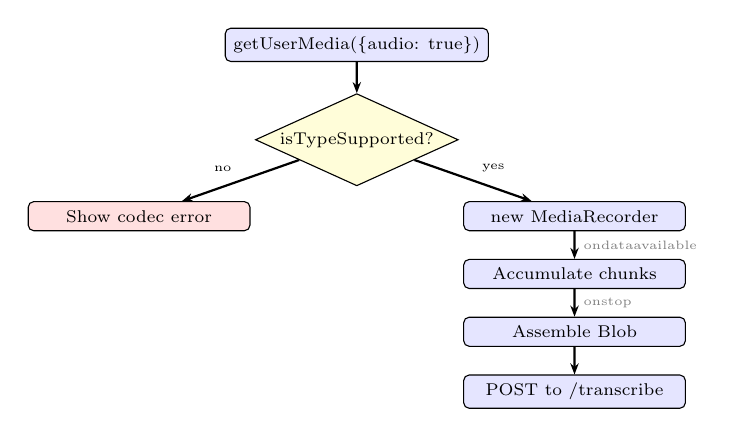
\begin{tikzpicture}[scale=0.88, every node/.style={transform shape},
        node distance=0.35cm,
        box/.style={draw, rounded corners=2pt, minimum width=3.2cm,
                    minimum height=0.42cm, font=\scriptsize, align=center},
        api/.style={box, fill=blue!10},
        check/.style={draw, diamond, aspect=2.2, font=\scriptsize,
                      align=center, fill=yellow!15, inner sep=1pt},
        err/.style={box, fill=red!12},
        arr/.style={-{Stealth[length=4pt]}, thick},
        lbl/.style={font=\tiny, text=gray},
    ]
        \node[api]   (gum)    {getUserMedia(\{audio: true\})};
        \node[check, below=0.45cm of gum] (sup)  {isTypeSupported?};
        \node[err,   below left=0.55cm and 0.8cm of sup]  (error) {Show codec error};
        \node[api,   below right=0.55cm and 0.8cm of sup] (rec)   {new MediaRecorder};
        \node[api,   below=0.4cm of rec]   (chunks) {Accumulate chunks};
        \node[api,   below=0.4cm of chunks](blob)   {Assemble Blob};
        \node[api,   below=0.4cm of blob]  (post)   {POST to /transcribe};

        \draw[arr] (gum) -- (sup);
        \draw[arr] (sup) -- node[above left, font=\tiny]{no} (error);
        \draw[arr] (sup) -- node[above right, font=\tiny]{yes} (rec);
        \draw[arr] (rec) -- node[right, lbl]{ondataavailable} (chunks);
        \draw[arr] (chunks) -- node[right, lbl]{onstop} (blob);
        \draw[arr] (blob) -- (post);
    \end{tikzpicture}
    \end{center}

    \vspace{0.2em}
    {\scriptsize The diamond is a hard gate --- recording never starts if the
    codec is unsupported. This prevents silent failures where the browser
    records in an unexpected format that the backend cannot transcode.}
\end{frame}


\begin{frame}{Server-Side Transcoding}
    \small
    The browser produces \texttt{webm/opus}. The model expects
    16\,kHz mono WAV. Transcoding is performed server-side by ffmpeg
    inside the container.

    \vspace{0.3em}
    \begin{itemize}\setlength{\itemsep}{2pt}
        \item The backend accepts five audio MIME types --- any format
              ffmpeg can decode is a valid input
        \item All inputs are normalized to the same output:
              16\,kHz sample rate, single channel, PCM WAV
        \item Adding a new input format requires only adding the MIME type
              to the allowlist --- zero frontend changes
        \item ffmpeg runs with a 30-second timeout to prevent hung processes
    \end{itemize}

    \vspace{0.2em}
    \begin{block}{Why Not Transcode in the Browser?}
        Keeping transcoding server-side means the frontend is format-agnostic.
        It sends whatever the \texttt{MediaRecorder} produces, and the
        backend normalizes. This isolates codec complexity to one place.
    \end{block}
\end{frame}


\begin{frame}{Server-Side Transcoding --- Diagram}
    \begin{center}
    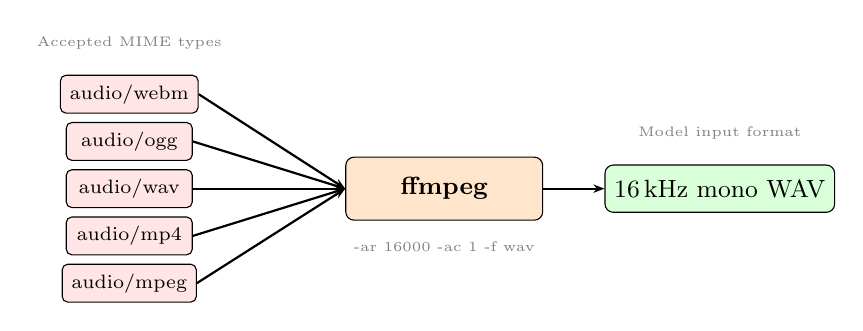
\begin{tikzpicture}[
        node distance=0.4cm,
        fmt/.style={draw, rounded corners=2pt, minimum width=1.6cm,
                    minimum height=0.42cm, font=\scriptsize, align=center,
                    fill=red!10},
        proc/.style={draw, rounded corners=3pt, minimum width=2.5cm,
                     minimum height=0.8cm, font=\small\bfseries,
                     align=center, fill=orange!20},
        outbox/.style={draw, rounded corners=3pt, minimum width=2.8cm,
                    minimum height=0.6cm, font=\small, align=center,
                    fill=green!15},
        arr/.style={-{Stealth[length=4pt]}, thick},
        lbl/.style={font=\tiny, text=gray},
    ]
        % Input formats
        \node[fmt] (webm) at (0, 0.0) {audio/webm};
        \node[fmt] (ogg)  at (0, -0.6) {audio/ogg};
        \node[fmt] (wav)  at (0, -1.2) {audio/wav};
        \node[fmt] (mp4)  at (0, -1.8) {audio/mp4};
        \node[fmt] (mp3)  at (0, -2.4) {audio/mpeg};

        % ffmpeg
        \node[proc] (ffmpeg) at (4.0, -1.2) {ffmpeg};

        % Output
        \node[outbox] (output) at (7.5, -1.2) {16\,kHz mono WAV};

        % Arrows
        \foreach \src in {webm, ogg, wav, mp4, mp3} {
            \draw[arr] (\src.east) -- (ffmpeg.west);
        }
        \draw[arr] (ffmpeg.east) -- (output.west);

        % Labels
        \node[lbl, above=0.2cm of webm] {Accepted MIME types};
        \node[lbl, above=0.2cm of output] {Model input format};
        \node[lbl, below=0.15cm of ffmpeg] {-ar 16000 -ac 1 -f wav};
    \end{tikzpicture}
    \end{center}

    \vspace{0.4em}
    {\scriptsize Five input formats funnel through a single normalization step.
    The model always receives identical input regardless of browser or
    source format. Safety bounds: 10\,MB cap, 60\,s duration, 30\,s timeout.}
\end{frame}


\begin{frame}{Inference}
    \small
    \texttt{faster-whisper} provides CTranslate2-optimized Whisper inference,
    running locally on the GPU with no external API calls.

    \vspace{0.2em}
    \begin{columns}[T]
        \begin{column}{0.48\textwidth}
            \textbf{Model configuration}
            \begin{itemize}\setlength{\itemsep}{0pt}\setlength{\parskip}{0pt}
                \item Model: \texttt{large-v3} (default)
                \item Device: CUDA (GPU)
                \item Compute type: \texttt{float16}
                \item Beam size: 5
                \item Fallback: \texttt{small} on CPU, \texttt{int8}
                      {\scriptsize\textit{(verified)}}
            \end{itemize}
        \end{column}
        \begin{column}{0.48\textwidth}
            \textbf{Runtime behavior}
            \begin{itemize}\setlength{\itemsep}{0pt}\setlength{\parskip}{0pt}
                \item Model loaded once at startup
                \item Held in GPU memory for lifetime
                \item Synchronous (blocks thread)
                \item Single-user --- no concurrency
                \item VAD filtering enabled
            \end{itemize}
        \end{column}
    \end{columns}

    \vspace{0.2em}
    {\footnotesize\textbf{Synchronous design:}
    \texttt{faster-whisper} blocks the thread during inference.
    Correct for single-user. Rework path: \texttt{asyncio.to\_thread()}
    or background task with polling (both change the API contract).}\par
\end{frame}


% =========================================================================
\section{Frontend}
% =========================================================================

\begin{frame}{Component Architecture}
    The frontend is a small React application with a clear separation
    between container logic, presentational components, and services.

    \vspace{0.6em}
    \begin{itemize}
        \item \textbf{App} is the sole container component --- it owns all state
              and orchestrates the record-transcribe-display flow
        \item \textbf{Recorder} and \textbf{Transcript} are presentational ---
              they receive props and emit callbacks, no internal state management
        \item \textbf{useRecorder} encapsulates the MediaRecorder lifecycle
              in a custom hook, keeping browser API complexity out of components
        \item \textbf{api.ts} is a thin service layer --- typed \texttt{fetch()}
              calls with error handling
    \end{itemize}

    \vspace{0.4em}
    \rmk The frontend has no routing, no global state library, and no
    build-time environment variables. Complexity is earned, not assumed.
\end{frame}


\begin{frame}{Component Architecture --- Diagram}
    \begin{center}
    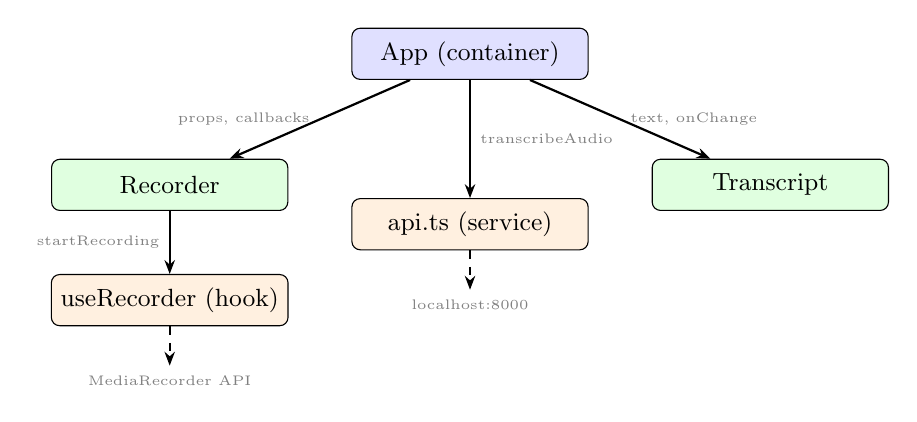
\begin{tikzpicture}[
        node distance=0.6cm,
        comp/.style={draw, rounded corners=3pt, minimum width=3cm,
                     minimum height=0.65cm, font=\small, align=center},
        container/.style={comp, fill=blue!12},
        present/.style={comp, fill=green!12},
        service/.style={comp, fill=orange!12},
        arr/.style={-{Stealth[length=5pt]}, thick},
        lbl/.style={font=\tiny, text=gray},
        boundary/.style={draw, dashed, rounded corners=5pt, gray, inner sep=8pt},
    ]
        % App
        \node[container] (app) {App (container)};

        % Components
        \node[present, below left=1cm and 0.8cm of app] (rec) {Recorder};
        \node[present, below right=1cm and 0.8cm of app] (trans) {Transcript};

        % Services
        \node[service, below=0.8cm of rec] (hook) {useRecorder (hook)};
        \node[service, below=1.5cm of app] (api) {api.ts (service)};

        % External
        \node[lbl, below=0.5cm of hook] (mic) {MediaRecorder API};
        \node[lbl, below=0.5cm of api] (backend) {localhost:8000};

        \draw[arr] (app) -- node[left, lbl]{props, callbacks} (rec);
        \draw[arr] (app) -- node[right, lbl]{text, onChange} (trans);
        \draw[arr] (rec) -- node[left, lbl]{startRecording} (hook);
        \draw[arr] (app) -- node[right, lbl]{transcribeAudio} (api);
        \draw[arr, dashed] (hook) -- (mic);
        \draw[arr, dashed] (api) -- (backend);
    \end{tikzpicture}
    \end{center}

    \vspace{0.2em}
    {\scriptsize \textcolor{blue!60}{Blue} = container (state owner),
    \textcolor{green!50!black}{Green} = presentational (stateless),
    \textcolor{orange!70}{Orange} = services (side effects).
    Dashed arrows = external system boundaries.}
\end{frame}


\begin{frame}{State Machine}
    The UI has five recording pipeline states plus a settings overlay.

    \vspace{0.4em}
    \begin{itemize}\setlength{\itemsep}{1pt}
        \item \textbf{idle} --- Ready. Record button enabled.
        \item \textbf{recording} --- Capturing audio. Button shows ``Stop'' (red).
        \item \textbf{processing} --- Audio sent to API. Button disabled.
        \item \textbf{done} --- Transcript in editable textarea. Copy button visible.
        \item \textbf{error} --- Error message displayed. User can retry.
    \end{itemize}

    \vspace{0.3em}
    \textbf{Settings overlay} is orthogonal to the pipeline ---
    a separate \texttt{settingsOpen: boolean}, not a sixth state.
    Accessible from idle, done, and error.
    Not accessible during recording or processing.

    \vspace{0.3em}
    Every state transition is triggered by a user action or an
    API response --- never by a timer or side effect.
    Hotkeys (\texttt{Ctrl+Shift+<key>}) trigger the same transitions
    as button clicks.
\end{frame}


\begin{frame}{State Machine --- Diagram}
    \begin{center}
    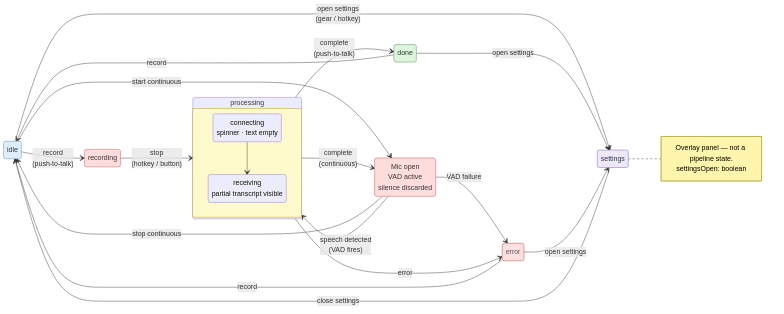
\includegraphics[width=\textwidth]{images/state-machine.png}
    \end{center}

    \vspace{0.2em}
    {\scriptsize The settings node is an overlay panel, not a pipeline state.
    Recording controls are inaccessible while settings is open.
    Both terminal states (done and error) loop back to idle on the next
    record action. Settings is accessible from any rest state.}
\end{frame}


% =========================================================================
\section{Security}
% =========================================================================

\begin{frame}{Threat Model}
    \small
    \begin{table}
    \centering
    \scriptsize
    \begin{tabular}{lll}
        \toprule
        \textbf{Asset} & \textbf{Sensitivity} & \textbf{Location} \\
        \midrule
        Microphone audio  & High  & Browser memory, temp file (transient) \\
        Transcript text   & High  & Browser memory, HTTP response \\
        Session metadata  & Low   & Container logs (durations, formats) \\
        Model weights     & None  & data/cache/ (public files) \\
        \bottomrule
    \end{tabular}
    \end{table}

    \vspace{0.2em}
    \textbf{Primary attack surfaces and mitigations:}
    \begin{itemize}\setlength{\itemsep}{1pt}
        \item \textbf{Upload endpoint} --- MIME validation, 10\,MB size cap,
              60\,s duration cap, 30\,s ffmpeg timeout
        \item \textbf{Temp storage} --- \texttt{try/finally} cleanup;
              dedicated directory; crash residuals monitored
        \item \textbf{CORS / origin} --- Restricted to localhost origins only;
              no wildcard
        \item \textbf{Dependencies} --- Pinned versions, weekly Dependabot scans
    \end{itemize}

    \vspace{0.2em}
    \nt Most likely failure: accidental LAN exposure via bind address change.
\end{frame}


\begin{frame}{Privacy --- Data Flow}
    \small
    The privacy model is defined by what data exists where, and for how long.

    \vspace{0.3em}
    \begin{itemize}\setlength{\itemsep}{2pt}
        \item Audio exists in three places: browser memory (during recording),
              HTTP transit (localhost only), and a temp file (seconds)
        \item The transcript exists in two places: HTTP response (localhost only)
              and the browser textarea (until page close)
        \item \textbf{Nothing is persisted server-side} --- the API is stateless
              between requests
        \item Operational logs contain only durations, formats, and detected
              language --- never content
    \end{itemize}

    \vspace{0.2em}
    \begin{block}{Network Boundary}
        API binds to \texttt{localhost:8000}. CORS restricted to
        \texttt{localhost:5173} and \texttt{127.0.0.1:5173}.
        Zero external network traffic at any point.
    \end{block}
\end{frame}


\begin{frame}{Privacy --- Data Flow Diagram}
    \begin{center}
    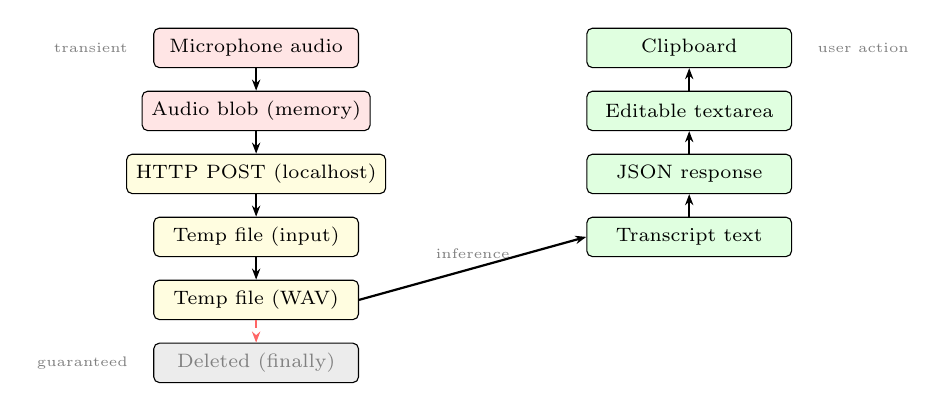
\begin{tikzpicture}[
        node distance=0.4cm,
        box/.style={draw, rounded corners=2pt, minimum width=2.6cm,
                    minimum height=0.5cm, font=\scriptsize, align=center},
        data/.style={box, fill=red!10},
        ephemeral/.style={box, fill=yellow!12},
        output/.style={box, fill=green!12},
        dead/.style={box, fill=gray!15, text=gray},
        arr/.style={-{Stealth[length=4pt]}, thick},
        delarr/.style={-{Stealth[length=4pt]}, thick, red!60, dashed},
        lbl/.style={font=\tiny, text=gray},
    ]
        % Audio path
        \node[data]      (mic)   at (0, 0) {Microphone audio};
        \node[data]      (blob)  at (0, -0.8) {Audio blob (memory)};
        \node[ephemeral] (http)  at (0, -1.6) {HTTP POST (localhost)};
        \node[ephemeral] (tmp1)  at (0, -2.4) {Temp file (input)};
        \node[ephemeral] (tmp2)  at (0, -3.2) {Temp file (WAV)};
        \node[dead]      (del)   at (0, -4.0) {Deleted (finally)};

        % Transcript path
        \node[output]    (text)  at (5.5, -2.4) {Transcript text};
        \node[output]    (resp)  at (5.5, -1.6) {JSON response};
        \node[output]    (area)  at (5.5, -0.8) {Editable textarea};
        \node[output]    (clip)  at (5.5, 0) {Clipboard};

        % Audio flow
        \draw[arr] (mic) -- (blob);
        \draw[arr] (blob) -- (http);
        \draw[arr] (http) -- (tmp1);
        \draw[arr] (tmp1) -- (tmp2);
        \draw[delarr] (tmp2) -- (del);

        % Inference to transcript
        \draw[arr] (tmp2.east) -- node[above, lbl]{inference} (text.west);

        % Transcript flow
        \draw[arr] (text) -- (resp);
        \draw[arr] (resp) -- (area);
        \draw[arr] (area) -- (clip);

        % Labels
        \node[lbl, left=0.2cm of mic] {transient};
        \node[lbl, left=0.2cm of del] {guaranteed};
        \node[lbl, right=0.2cm of clip] {user action};
    \end{tikzpicture}
    \end{center}

    \vspace{0.1em}
    {\scriptsize \textcolor{red!60}{Red} = sensitive audio (transient).
    \textcolor{yellow!70!black}{Yellow} = ephemeral intermediate.
    \textcolor{green!50!black}{Green} = transcript output (user-controlled).
    \textcolor{gray}{Gray} = deleted. Red dashed = deletion point.}
\end{frame}


\begin{frame}{Operational Telemetry}
    The system logs \textit{operations}, not \textit{content}.
    Every event includes an ISO 8601 timestamp via \texttt{structlog}.

    \vspace{0.4em}
    \begin{table}
    \centering
    \scriptsize
    \begin{tabular}{ll}
        \toprule
        \textbf{Event} & \textbf{Fields} \\
        \midrule
        \texttt{model download started}  & model name, device \\
        \texttt{model download complete} & duration \\
        \texttt{transcode started}       & input MIME type \\
        \texttt{transcode complete}      & output format, duration \\
        \texttt{inference started}       & audio file path \\
        \texttt{inference complete}      & duration, detected language \\
        \bottomrule
    \end{tabular}
    \end{table}

    \vspace{0.4em}
    \begin{itemize}
        \item All output is structured and greppable from container logs
        \item Log level defaults to \texttt{info}; adjustable via \texttt{LOG\_LEVEL}
        \item Transcript content is \textbf{never} logged at any level ---
              this is a hard requirement, not a convention
    \end{itemize}
\end{frame}


% =========================================================================
\section{Development}
% =========================================================================

\begin{frame}[fragile]{Workflow \& Tooling}
    \small
    \textbf{Development environment:}
    WSL2 Linux filesystem, VS Code with WSL extension,
    Docker Desktop with WSL2 backend, Chrome for testing.

    \vspace{0.3em}
    \textbf{Makefile targets:}
    \vspace{0.1em}

    \begin{table}
    \centering
    \small
    \begin{tabular}{ll}
        \toprule
        \textbf{Command} & \textbf{Purpose} \\
        \midrule
        \texttt{make dev}       & Start API container + frontend dev server \\
        \texttt{make build}     & Build the API Docker image \\
        \texttt{make test}      & Run all tests (pytest + vitest) \\
        \texttt{make gpu-check} & Verify GPU/Docker readiness \\
        \bottomrule
    \end{tabular}
    \end{table}

    \vspace{0.3em}
    \textbf{Smoke test} (fastest full-stack feedback loop):
    \begin{lstlisting}[language=bash]
bash ops/scripts/smoke_test.sh ops/scripts/test.mp3
    \end{lstlisting}
    Tests \texttt{GET /health} and \texttt{POST /transcribe} against the
    running API with a real audio file.
\end{frame}


\begin{frame}{Testing Strategy}
    \small
    \begin{columns}[T]
        \begin{column}{0.48\textwidth}
            \textbf{Backend (pytest)}
            \begin{itemize}\setlength{\itemsep}{0pt}
                \item Health endpoint responses
                \item MIME type validation
                \item Codec parameter stripping
                \item File size rejection
                \item Missing file handling
            \end{itemize}
            \vspace{0.2em}
            {\scriptsize Runs inside Docker container\\(requires faster-whisper imports)}
        \end{column}
        \begin{column}{0.48\textwidth}
            \textbf{Frontend (vitest)}
            \begin{itemize}\setlength{\itemsep}{0pt}
                \item Record button state transitions
                \item Transcript textarea rendering
                \item Copy-to-clipboard action
                \item Loading state display
                \item Text edit callback
            \end{itemize}
            \vspace{0.2em}
            {\scriptsize Runs on host via Node.js\\(jsdom environment)}
        \end{column}
    \end{columns}

    \vspace{0.3em}
    \begin{block}{Test Philosophy}
        Test the happy path plus the obvious failure boundaries.
        Do not overbuild the test matrix before the first usable
        version exists. The smoke test script catches integration
        failures that unit tests cannot.
    \end{block}
\end{frame}


% =========================================================================
\section{Roadmap}
% =========================================================================

\begin{frame}{v1 Scope}
    \small
    \textbf{v1 is intentionally narrow.} The entire product:

    \vspace{0.3em}
    \begin{enumerate}\setlength{\itemsep}{0pt}
        \item Record one utterance
        \item Send it to a local transcription API
        \item Return transcript text
        \item Show it in an editable text area
        \item Copy the result to clipboard
    \end{enumerate}

    \vspace{0.2em}
    \textbf{Explicit non-goals for v1:}
    \begin{multicols}{2}
    \begin{itemize}\setlength{\itemsep}{0pt}
        \item Continuous dictation
        \item Live streaming partials
        \item Multi-user deployment
        \item Async job queues
        \item Background workers
        \item Reverse proxies
        \item Desktop packaging
        \item Grammar LLM integration
    \end{itemize}
    \end{multicols}

    \vspace{-0.2em}
    \begin{center}
    \textit{Ship v1 small. Earn the right to make it bigger.}
    \end{center}
\end{frame}


% =========================================================================
\section{Interaction Model}
% =========================================================================

\begin{frame}{v2.0 --- Hotkeys + Settings}
    \small
    \textbf{Hotkey system} --- keyboard shortcuts for recording control,
    copy, clear, and settings toggle. All use \texttt{Ctrl+Shift+<key>}
    modifier to avoid conflicts with the editable textarea and Chrome
    built-in bindings.

    \vspace{0.3em}
    \begin{table}
    \centering\small
    \begin{tabular}{@{} l l @{}}
        \toprule
        \textbf{Hotkey} & \textbf{Action} \\
        \midrule
        \texttt{Ctrl+Shift+Space} & Toggle recording \\
        \texttt{Ctrl+Shift+Y}     & Copy transcript \\
        \texttt{Ctrl+Shift+X}     & Clear transcript \\
        \texttt{Ctrl+Shift+S}     & Toggle settings panel \\
        \bottomrule
    \end{tabular}
    \end{table}

    \vspace{0.3em}
    \textbf{Settings panel} --- model selection (swap between
    \texttt{large-v3} and \texttt{small} at runtime without editing
    \texttt{.env}). Model swap is full-stack: backend endpoint with
    threading lock, VRAM cleanup, and graceful fallback.
\end{frame}


\begin{frame}{v2.0 --- Model Swap Architecture}
    \small
    Runtime model selection requires a backend endpoint and safe reload logic.

    \vspace{0.3em}
    \begin{itemize}\setlength{\itemsep}{2pt}
        \item \texttt{GET /models} --- returns available models
              (configured via \texttt{WHISPER\_AVAILABLE\_MODELS} env var)
        \item \texttt{POST /models/swap} --- accepts model name,
              acquires threading lock, loads new model, frees old VRAM
        \item Swap blocks inference during reload (seconds).
              Frontend shows loading state; record button disabled
        \item If swap fails, old model remains loaded --- no degradation
        \item Regular \texttt{def} endpoint (not \texttt{async def}) ---
              runs in thread pool, keeps event loop alive for health checks
    \end{itemize}

    \vspace{0.2em}
    \begin{block}{Available Models}
        Intentionally limited to models declared in
        \texttt{WHISPER\_AVAILABLE\_MODELS}.
        No auto-discovery, no surprise downloads.
    \end{block}
\end{frame}


\begin{frame}{v2 Roadmap}
    \small
    \begin{columns}[T]
        \begin{column}{0.48\textwidth}
            \textbf{v2.0} (complete)
            \begin{itemize}\setlength{\itemsep}{0pt}
                \item Hotkey system
                \item Settings panel (model selection)
                \item State machine diagram update
            \end{itemize}

            \vspace{0.2em}
            \textbf{v2.1}
            \begin{itemize}\setlength{\itemsep}{0pt}
                \item Streaming (WebSocket)
                \item Voice activity detection (VAD)
            \end{itemize}
        \end{column}
        \begin{column}{0.48\textwidth}
            \textbf{v2.2}
            \begin{itemize}\setlength{\itemsep}{0pt}
                \item Continuous recording mode
                \item Silence-based segmentation
                \item Recording mode toggle in settings
            \end{itemize}

            \vspace{0.2em}
            \textbf{v2.3}
            \begin{itemize}\setlength{\itemsep}{0pt}
                \item Voice command vocabulary
                \item Stop, submit, redo, clear phrases
            \end{itemize}
        \end{column}
    \end{columns}

    \vspace{0.3em}
    \textbf{v3} --- Desktop packaging (Tauri). Global hotkeys.
    Direct injection into focused application. No Docker dependency.
\end{frame}


\end{document}
